\documentclass[9pt]{extarticle}
\usepackage{spconf,amsmath,graphicx}
\usepackage{algorithm}
\usepackage{algpseudocode}
\usepackage{amssymb}
\usepackage{amsthm}
\usepackage{xcolor}
\usepackage{caption}
\captionsetup{font=small, labelfont=bf}
\usepackage{enumitem}
\usepackage{hyperref}
\newtheorem{theorem}{Theorem}
\newtheorem{lemma}{Lemma}
\newtheorem{proposition}{Proposition}
\newtheorem{corollary}{Corollary}
\newtheorem{assumption}{Assumption}
 % smaller font inside algorithms
\makeatother
\algrenewcommand\algorithmicrequire{\textbf{In:}}
\algrenewcommand\algorithmicensure{\textbf{Out:}}
\algrenewcommand\algorithmicindent{0.8em}
\newcommand{\dk}[1]{\textbf{\textcolor{red}{ {DK: #1}}}}
\theoremstyle{definition}
\newtheorem{definition}[theorem]{Definition}
\newtheorem{example}[theorem]{Example}
\newtheorem{remark}[theorem]{Remark}
\newtheorem{notation}[theorem]{Notation}
% Notation convenience (optional)
\newcommand{\hadam}{\circ}
\newcommand{\ones}{\mathbf{1}}
\allowdisplaybreaks
% spconf.sty's \@sect override has no run-in branch, so the standard \paragraph
% errors (undefined \@svsechd); use a plain unnumbered run-in heading instead.
\renewcommand{\paragraph}[1]{\par\medskip\noindent{\bf #1}\hspace{0.5em}\ignorespaces}
\hyphenation{op-tical net-works semi-conduc-tor}
\begin{document}
\title{Optimally Transport Weighted Stochastic Gradient Descent to Mitigate Distribution Shift\vspace{-8pt}}
% make the title area
\maketitle

\begin{abstract}
Stochastic gradient descent implicitly assumes that mini-batches are exchangeable draws from a fixed population, but real datasets are often organized into critical groups, such as demographic categories, recording sites, or data sources, whose relative importance in the objective may need to be set explicitly rather than inherited from raw sample counts. This is straightforward when every group can appear in every batch; it breaks down when batches can only reveal a subset of groups at a time, which is the rule rather than the exception whenever collection logistics, storage layout, or access constraints determine which groups can co-occur. Naive fixes, such as fixed reweighting or oversampling, either ignore which groups a given batch can actually show or inflate variance and discard data. We propose a fair stochastic gradient descent framework that treats per-batch reweighting as a masked optimal transport problem, coupling the distribution over observable batch patterns to a target group distribution through a support mask determined by which groups can co-occur. Solving this transport problem yields per-batch weights that make the resulting stochastic gradient exactly unbiased for the target objective whenever a feasible transport plan exists, and a classical max-flow/min-cut feasibility condition, specialized to our masked setting, characterizes exactly when it does. We show the resulting projected algorithm converges at the standard rate for convex objectives, and that when exact feasibility fails, an entropy-regularized projection recovers the closest achievable target distribution together with an explicit, controllable bound on the resulting bias. We validate the approach, instantiated as FedAVOT, on income classification with demographic fairness metrics and on age regression under a realistic mismatch between how often a group is observable and how much it should count, where it tracks full-coverage performance whenever the underlying transport problem is feasible, improves on the uniform batch average by a margin that a closed-form feasibility diagnostic predicts before training, and remains stable in regimes where the standard fixed-multiplier correction diverges.
\end{abstract}
\section{Introduction}

Empirical risk minimization treats every training example as interchangeable, but many datasets carry group structure that the learner is expected to respect: demographic attributes in fairness-sensitive applications, subject or site identity in clinical and scientific data, device or sensor type in heterogeneous sensing, or domain label in multi-source data. When the objective is meant to weight these groups according to some target distribution, for instance uniformly across demographic groups regardless of their prevalence in the data, the standard fix is to reweight the loss or resample the data so that the empirical group frequencies match the target. This works cleanly when a mini-batch can, in principle, contain any group; the reweighting reduces to a fixed multiplier per group.

That assumption fails whenever batches are constrained to show only a subset of groups at a time. Streaming pipelines with bounded buffers deliver whichever groups happen to be resident; sensor and measurement networks return data only from the sites reachable at that moment; records held under access or privacy restrictions can be read only in permitted combinations; and in any pipeline where a batch is assembled from a few sources at a time, the batch is by construction restricted to whichever groups those sources carry. In these settings, a fixed per-group multiplier is not well defined, because the same group can appear alongside different partners from one iteration to the next, and some target distributions may not be achievable at all under the batch structure actually realized.

We address this by casting per-batch reweighting as a transport problem: probability mass must move from the distribution over observable batch patterns to the desired target distribution over groups, subject to a combinatorial mask that only allows mass to flow between a batch pattern and the groups it actually contains. Unlike classical optimal transport, there is no cost to minimize; the only question is feasibility, which admits a clean max-flow/min-cut characterization obtained by specializing classical flow-feasibility results~\cite{fordfulkerson1962flows,hall1935representatives} to the batch-sampling mask. When feasible, the resulting transport plan gives per-batch weights that make the stochastic gradient exactly unbiased for the target objective, and we prove the associated projected SGD algorithm converges at the standard $O(1/\sqrt{T})$ rate for convex objectives. When infeasible, for instance, because certain groups never co-occur in a batch, we show that an entropy-regularized projection still returns a well-defined, feasible surrogate target distribution, and we bound the resulting suboptimality by the same convergence rate plus an explicit, tunable bias term governed by how far the surrogate had to move from the intended target.
\section{Transport-Weighted SGD with Subset Sampling: Setup and Convergence}
We begin by formalizing the optimization setup, followed by the probabilistic and geometric interpretation of the proposed transport-weighted sampling procedure. Our goal is to provide a unifying view of mini-batch sampling and fairness weighting through a transport-theoretic lens.
In many practical settings, the data exhibit distinct \emph{critical groups}, such as demographic categories, device types, or environments, which we denote by $\mathcal{K}=\{K_1,\ldots,K_m\}$, where each $K_j\subset\mathcal{X}$ is a partition of the feature space. Each datapoint $x_i$ belongs to exactly one critical group $K_j$.

To correct this imbalance, we define a \emph{target group measure} $\mu=(\mu_1,\ldots,\mu_m)$ over $\mathcal{K}$, representing the desired weighting (e.g., uniform or risk-adjusted). The corresponding fair optimization objective becomes:
\begin{equation}\label{eq:fair-obj}
\boxed{\min_{\theta\in \Theta}\ \sum_{j=1}^{m}\mu_j\,\mathbb{E}_{(x,y)\in K_j}\left[\ell(f_\theta(x),y)\right]}.
\end{equation}
When $\mu=\nu$, this reduces to standard ERM; otherwise, it enforces fairness or domain alignment by up/down-weighting subgroups. Naïve oversampling or undersampling approximates this by modifying the data distribution, but these techniques may increase variance or discard data~\cite{buda2018systematic, he2009learning}.

In practice, optimization proceeds via stochastic gradient descent (SGD). At iteration $t$, a random subset (mini-batch) $\xi_t\subset\{1,\ldots,N\}$ is drawn \emph{without replacement}. Let $\mathcal{A}_1,\ldots,\mathcal{A}_{2^m-1}$ denote all non-empty subsets of $\mathcal{K}$ that may appear in a batch, and let $q_j$ be the probability that the active batch at iteration $t$ contains exactly the subgroup pattern $\mathcal{A}_j$.
Throughout the analysis we treat $q$ as known; when it is not available in closed form, it can be estimated offline by Monte Carlo simulation of the batch sampler, which is how our experiments obtain it (Section~\ref{sec:experiments}).
\paragraph{Weighted Gradient Aggregation.}
When the mini-batch $\xi_t$ belongs to $\mathcal{A}_j$, each group $i\in\mathcal{A}_j$ contributes a normalized proportion $Y[i,j]$ to the aggregated gradient. The joint allocation of group mass is given by:
\[
T[i,j] = q_j\,Y[i,j],
\]
representing the amount of probability mass transported from event $j$ (subset $\mathcal{A}_j$) to group $i$.

The weight assignment must satisfy:
\begin{align}\label{eq:constraints}
    &\sum_{j}T[i,j]=p_i=\mu_i, && \forall i, \nonumber\\
    &\sum_{i}T[i,j]=q_j, && \forall j, \nonumber\\
    &T[i,j]=0, && i\notin\mathcal{A}_j, \nonumber\\
    &T[i,j]\ge0, && \forall (i,j),
\end{align}
where the support mask $\mathcal{E}=\{(i,j)\mid i\in\mathcal{A}_j\}$ enforces feasible interactions between groups and subset events. These are exactly the marginal and non-negativity constraints of a \emph{masked optimal transport (MOT)} problem:
\begin{equation}\label{eq:mot}
T\mathbf{1}_M=p, \quad \mathbf{1}_N^\top T=q, \quad T\ge0, \quad \operatorname{supp}(T)\subseteq \mathcal{E}.
\end{equation}
Feasibility of~\eqref{eq:mot} admits a simple max-flow/min-cut characterization: the following theorem specializes the classical supply--demand feasibility theorem of Ford and Fulkerson~\cite{fordfulkerson1962flows}, whose bipartite ancestor is Hall's marriage theorem~\cite{hall1935representatives}, to the membership mask $\mathcal{E}$.
\begin{theorem}[\textbf{Feasibility of Masked OT}~\cite{fordfulkerson1962flows,hall1935representatives}]
\label{thm:feasibility}
Let $I\subseteq[N]$, $\mathcal{N}(I):=\{j\mid \exists i\in I,\ (i,j)\in\mathcal{E}\}$, and $\mathcal{S}(I):=\{j\mid \mathcal{A}_j\subseteq I\}$. Then~\eqref{eq:mot} is feasible iff
\begin{equation}\label{eq:feasibility}
\sum_{j\in\mathcal{S}(I)} q_j \le \sum_{i\in I} p_i \le \sum_{j\in\mathcal{N}(I)} q_j, \quad \forall I\subseteq[N].
\end{equation}
\end{theorem}

Given feasibility, $T$ can be computed efficiently using the \textit{Iterative Proportional Fitting Procedure (IPFP)}~\cite{sinkhorn1967concerning, knight2008sinkhorn}, also known as \textit{Sinkhorn scaling}, which alternates between row and column normalization.
If $p$ and $q$ satisfy~\eqref{eq:feasibility}, IPFP converges to a feasible solution of~\eqref{eq:mot}~\cite{sinkhorn1967concerning, knight2008sinkhorn}.
\section{Convergence of Projected Transport-Weighted SGD (FedAVOT)}
We analyze the projected SGD algorithm that uses the transport weights described earlier to produce an unbiased stochastic gradient of the \emph{target} (fair) objective
\begin{equation}\label{eq:target-objective}
F(\theta) \;:=\; \sum_{i=1}^m \mu_i \,\mathbb{E}_{(x,y)\sim \mathcal{D}_i}\!\big[\ell\!\left(f_\theta(x),y\right)\big],
\qquad \theta\in\Theta,
\end{equation}
where $\mathcal{D}_i$ is the (unknown) data distribution within group $K_i$ and $(\mu_1,\dots,\mu_m)$ is the desired target measure over groups. We assume $F$ is convex on a nonempty, closed, convex, and compact constraint set $\mathcal{C}\subseteq\Theta$; the projection $\Pi_{\mathcal{C}}$ is therefore well-defined. Let $\theta^\star\in\arg\min_{\theta\in\mathcal{C}}F(\theta)$.
\paragraph{Sampling and weighting.}
At iteration $t$, a mini-batch $\xi_t$ is drawn (without replacement) from the dataset; let $j_t\in\{1,\dots,M\}$ index the \emph{active group-subset} $\mathcal{A}_{j_t}\subseteq\{1,\dots,m\}$ observed in that batch. As in the setup, let $q_j=\mathbb{P}(j_t=j)$ be the probability of subset $\mathcal{A}_j$ under the sampling scheme, and let $Y[i,j]\ge 0$ denote the normalized contribution (weight) assigned to group $i$ when the active subset is $j$ (so $Y[i,j]=0$ if $i\notin\mathcal{A}_j$). Define $T[i,j]=q_j Y[i,j]$ and recall the masking and marginal constraints
\begin{equation}\label{eq:marginals}
\sum_{j=1}^M T[i,j]=\mu_i,\quad \sum_{i=1}^m T[i,j]=q_j,\quad T[i,j]=0 \ \text{if}\ i\notin\mathcal{A}_j.
\end{equation}
Hence $\sum_{j} q_j Y[i,j]=\mu_i$ for all $i$.
Within batch $\xi_t$, we compute the (per-sample) gradients and aggregate them group-wise, then scale by the transport weights so that the stochastic gradient estimator is
\begin{equation}\label{eq:gt}
g_t \;=\; \sum_{i\in\mathcal{A}_{j_t}} Y[i,j_t]\;\widehat{g}_{t,i},
\qquad
\text{with}\quad
\widehat{g}_{t,i} \;=\; \frac{1}{|\xi_t\cap K_i|}\sum_{(x,y)\in \xi_t\cap K_i} \nabla_\theta \ell\!\left(f_{\theta_t}(x),y\right).
\end{equation}
(When $|\xi_t\cap K_i|=0$, we interpret $\widehat{g}_{t,i}$ as $0$ and $Y[i,j_t]=0$ by construction.)
\begin{assumption}[\textbf{Bounded second moment}]\label{assump:gradient_bound}
There exists $G>0$ such that for all $\theta\in\mathcal{C}$,
\[
\mathbb{E}\!\left[\|g_t\|^2 \,\big|\, \theta_t=\theta\right] \;\le\; G^2.
\]
\end{assumption}
\begin{lemma}[\textbf{Unbiasedness}]\label{lem:unbiased}
Under \eqref{eq:marginals}, the estimator $g_t$ in \eqref{eq:gt} is conditionally unbiased:
\[
\mathbb{E}\!\left[g_t \,\big|\, \theta_t\right] \;=\; \nabla F(\theta_t).
\]
\end{lemma}
\begin{proof}
Condition on $\theta_t$, take expectation over $j_t\sim q$, and use $\sum_j q_j Y[i,j]=\mu_i$ from \eqref{eq:marginals}.
\end{proof}
\subsection{Convergence Rate}
Let $D:=\sup_{\theta,\theta'\in\mathcal{C}}\|\theta-\theta'\|$ denote the (finite) diameter of $\mathcal{C}$ in the Euclidean norm. Consider the averaged iterate $\bar{\theta}_T := \frac{1}{T}\sum_{t=1}^T \theta_t$.
\begin{theorem}[\textbf{Projected FedAVOT: $O(1/\sqrt{T})$ suboptimality}]\label{thm:main}
Suppose $F$ is convex on $\mathcal{C}$, Assumption~\ref{assump:gradient_bound} holds, and the gradient estimator $g_t$ is unbiased (Lemma~\ref{lem:unbiased}). For any step sizes $\{\eta_t\}_{t=1}^T$,
\begin{equation}\label{eq:key-bound}
\mathbb{E}\!\left[F(\bar{\theta}_T) - F(\theta^\star)\right]
\;\le\;
\frac{\|\theta_1-\theta^\star\|^2}{2\sum_{t=1}^T \eta_t}
\;+\;
\frac{G^2}{2T}\sum_{t=1}^T \eta_t.
\end{equation}
In particular, with the choice $\eta_t \equiv \eta = \frac{D}{G\sqrt{T}}$,
\begin{equation}\label{eq:rate}
\mathbb{E}\!\left[F(\bar{\theta}_T) - F(\theta^\star)\right]
\;\le\; \frac{DG}{\sqrt{T}}.
\end{equation}
\end{theorem}
\begin{proof}[Proof sketch]
Non-expansiveness of $\Pi_{\mathcal{C}}$ gives $\|\theta_{t+1}-\theta^\star\|^2 \le \|\theta_t-\theta^\star\|^2 - 2\eta_t \langle g_t, \theta_t-\theta^\star\rangle + \eta_t^2 \|g_t\|^2$; taking conditional expectation, applying Lemma~\ref{lem:unbiased}, convexity and Assumption~\ref{assump:gradient_bound}, telescoping over $t$, and using Jensen's inequality on $\bar{\theta}_T$ gives \eqref{eq:key-bound}; the constant step $\eta=D/(G\sqrt{T})$ gives \eqref{eq:rate}. The same rate holds for $\eta_t=\eta_0/\sqrt{t}$ up to constants.
\end{proof}
\subsection{Infeasible Masks and Entropy-Regularized Projection of Target Marginals}
\label{subsec:infeasible}
The subset constraints \eqref{eq:feasibility} ensure that the target weights $p=\mu$ are realizable given the batch-sampling structure (mask) $\mathcal{E}$.
However, in practice, these conditions are often violated, especially in heterogeneous settings where data coverage is incomplete or unbalanced across groups.
For example, one may wish to assign uniform importance across the $m$ groups, $p_i = 1/m$, while the batch law $q$ is highly skewed, or certain groups rarely co-occur in a single batch.
In such cases, the masking constraints prohibit exact satisfaction of $T\mathbf{1}=p$ and $\mathbf{1}^\top T=q$, rendering \eqref{eq:mot} \emph{infeasible}.
\subsubsection{Entropy-Regularized Projection and Feasible Surrogate Objective}
When \eqref{eq:feasibility} fails, we consider the entropy-regularized masked OT problem:
\begin{equation}\label{eq:entropic-mot-failure}
\min_{T\ge 0}\;\;\sum_{i,j} C[i,j]\,T[i,j] \;+\; \varepsilon \sum_{i,j} T[i,j]\log T[i,j]
\quad\text{s.t.}\quad \mathbf{1}^\top T=q^\top,\;\operatorname{supp}(T)\subseteq\mathcal{E}.
\end{equation}
This formulation is strictly convex and admits a unique minimizer $T_\varepsilon$~\cite{cuturi2013sinkhorn,peyre2019computational}.
Its row sums,
\begin{equation}\label{eq:phat-failure}
\hat{p} \;:=\; T_\varepsilon \mathbf{1},
\end{equation}
represent the \emph{closest feasible marginals} in the sense of KL projection~\cite{csiszar1975ipr}.
Operationally, Sinkhorn or IPFP iterations converge to $T_\varepsilon$, even in the absence of exact feasibility, yielding a reweighted marginal $\hat{p}$ satisfying $\hat{p}\in\mathcal{R}(q,\mathcal{E})$, where $\mathcal{R}(q,\mathcal{E})$ denotes the set of realizable row marginals under the mask and fixed $q$.
However, since $F_p$ and $F_{\hat{p}}$ differ, the total deviation decomposes as:
\begin{align}
\mathbb{E}\!\left[F_p(\bar{\theta}_T) - F_p(\theta^\star)\right]
&\le \frac{DG}{\sqrt{T}} \;+\; 2B\,\|p-\hat{p}\|_1,
\label{eq:infeasible-rate}
\end{align}
with the second term representing an irreducible \emph{statistical bias} induced by the mismatch between desired and realizable group marginals.
This term persists regardless of $T$ and quantifies the structural error caused by infeasibility.
\section{Experiments}
\label{sec:experiments}
\paragraph{Common Protocol for the Availability-Mismatch Experiments}
In the experiments of this section the batch structure is availability-driven: at each iteration the sampler exposes an active set $S^t$ of $K$ of the $m$ critical groups, drawn without replacement with probabilities proportional to per-group availability weights $r$, which induces the batch law $q$ over the $M=\binom{m}{K}$ observable patterns $\mathcal{A}_j$; we estimate $q$ from $10^6$ Monte Carlo draws of this sampler ($4\times10^5$ in the synthetic study) and fit the plan $T$ by Sinkhorn scaling under the membership mask, normalizing each column to the FedAVOT weights $Y[i,j]=T[i,j]/q_j$. Every exposed group performs $H=5$ local epochs of full-batch gradient descent on its own data before aggregation, with the decaying step size $\eta_t = \eta_\theta/(1+t/T_0)$, $T_0 = 1000$, and four aggregation rules are updated in parallel from the same draw $S^t$, so their trajectories are directly comparable: FedAVOT; the \emph{uniform average} $\frac{1}{K}\sum_{i\in S^t}\theta_i$ over the exposed groups, which ignores importance altogether and is the natural baseline; the fixed-multiplier $m/K$ correction; and the full-coverage reference. We report the importance-weighted objective $F(\theta^t)$ per iteration (squared loss for the regression tasks, cross-entropy for Adult); final values average the last $500$ iterations and are given as mean $\pm$ standard deviation over seeds. Recall that instantiating the feasibility condition~\eqref{eq:feasibility} of Theorem~\ref{thm:feasibility} at the singleton sets $I=\{i\}$ yields the per-group requirement $p_i \le \pi_i := \sum_{j:\, i \in \mathcal{A}_j} q_j$; this ceiling is the operative condition in our designs, and in every regime we call feasible, IPFP converges to machine precision, certifying that the remaining inequalities of~\eqref{eq:feasibility} hold as well. We quantify infeasibility as the importance mass $\sum_{i:\, p_i > \pi_i} p_i$ held by violating groups, and design $r$ to place each experiment on a chosen side of this condition. Throughout, the \emph{full-coverage reference} is the idealized run in which every batch reveals all $m$ groups and each is weighted by its target importance $p_i$; it is the objective value the transport is trying to recover, not a competing method.
\paragraph{IMDb-Wiki Age Regression Under Availability--Importance Mismatch} We take celebrity identity as the group attribute and use the first $m=100$ identities with at least $30$ training images as the critical groups, each holding $30$ images represented by $128$-dimensional face embeddings from a pretrained ResNet; the task is linear regression of mean-centered age on the embedding, with $K=3$, learning rate $\eta_\theta=10^{-2}$, $4000$ iterations, and $5$ seeds. All availability regimes share the same cubic importance $p_i \propto (m{+}1{-}i)^3$ and differ only in $r$, which we parametrize as $r_i \propto i^{\beta}$. The \emph{uniform} regime ($\beta=0$) is the default one gets when every identity is equally observable; even so, the cubic target is infeasible for the $9$ most important groups ($\max_i p_i/\pi_i = 1.30$), which hold $31\%$ of the importance mass. Increasing $\beta$ tilts availability against importance, up to the \emph{mirrored} regime $\beta=3$, where $r$ is the exact mirror image of $p$ and $41$ of $100$ groups holding approximately $88\%$ of the importance mass are infeasible; we sweep $\beta \in \{0, 0.5, 1, 1.5, 2, 3\}$. In the \emph{aligned} regime, $r_i \propto m{+}1{-}i$ is a linear skew in the same direction as $p$; feasibility then holds for every group ($\max_i p_i/\pi_i = 0.66$), while the cubic-versus-linear shape mismatch still requires nontrivial transport reweighting.
\paragraph{Adult Income Classification: A Group-Uniform Fairness Target Across Race}
The Adult (Census Income) dataset, derived from the 1994 U.S.\ Census, contains $48{,}842$ individuals with $14$ demographic and socioeconomic attributes; the task is binary classification of whether income exceeds \$50{,}000, trained by logistic regression under the cross-entropy loss on one-hot-encoded categorical and standardized numerical features ($d=109$ including an intercept). The critical groups are homogeneous with respect to race: each of the $m=100$ groups holds $30$ samples from exactly one race category, and the number of groups per category is proportional to that category's prevalence in the data (White/Black/Asian-Pac-Islander/Amer-Indian-Eskimo/Other $= 85/10/3/1/1$). The importance distribution is the fairness target itself: uniform across the five race categories, $1/5$ per category divided equally among that category's groups, so groups drawn from the smallest categories carry individual importance up to $p_i = 0.2$. Availability defines two regimes under the common protocol. In the \emph{prevalence} regime every group is equally observable ($r$ uniform), the default one gets when exposure mirrors data prevalence; the five groups belonging to the three smallest race categories then hold $60\%$ of the importance mass against inclusion probabilities $\pi_i \approx K/m = 0.03$, so the fairness target is infeasible purely because the categories are imbalanced. In the \emph{aligned} regime availability is proportional to importance ($r \propto p$), which restores feasibility; the family $r \propto p^{\beta}$, $\beta \in \{0, 0.25, 0.5, 0.75, 1\}$, interpolates between the two. We train with $K=3$, $\eta_\theta = 0.1$, $H=5$, $4000$ iterations, and $5$ seeds.
% ---------------------------------------------------------------- figures
\begin{figure}[t]
  \centering
  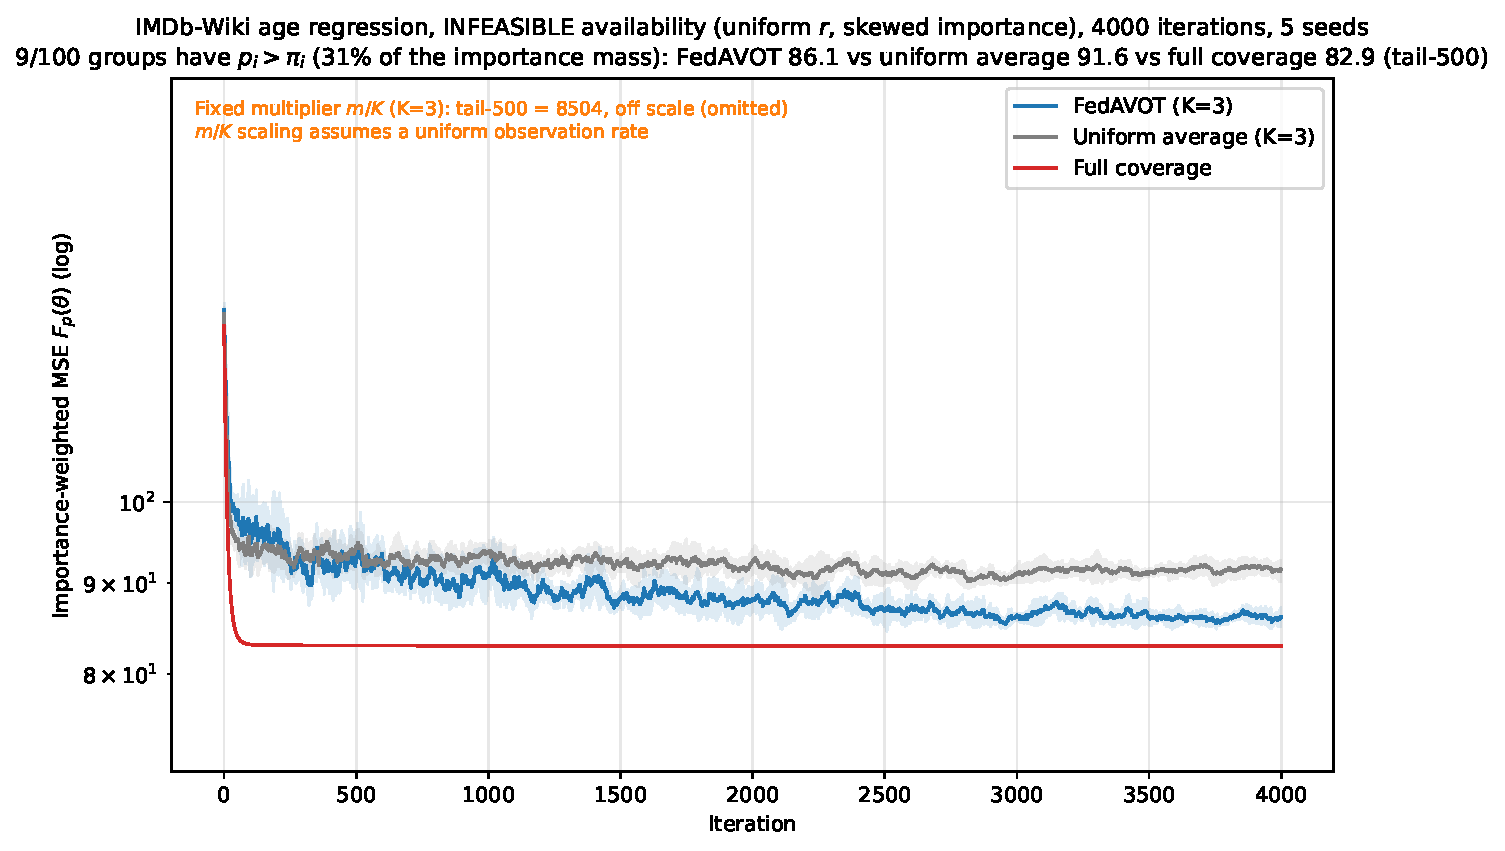
\includegraphics[width=0.6\linewidth]{imdbwiki_infeasible_K3_4000rounds_decay.pdf}
  \caption{IMDb-Wiki age regression under uniform availability ($\beta=0$;
  $p_i \propto (m{+}1{-}i)^3$, $r$ uniform; $5$ seeds, shaded $\pm 1$ std).
  The cubic target is infeasible for $9$ groups holding $31\%$ of the
  importance mass, yet FedAVOT ($86.1$) recovers two thirds of the gap
  between the uniform average ($91.6$) and full coverage ($82.9$); the
  fixed-multiplier correction is unstable and off scale.}
  \label{fig:imdb-infeasible}
\end{figure}
\begin{figure}[t]
  \centering
  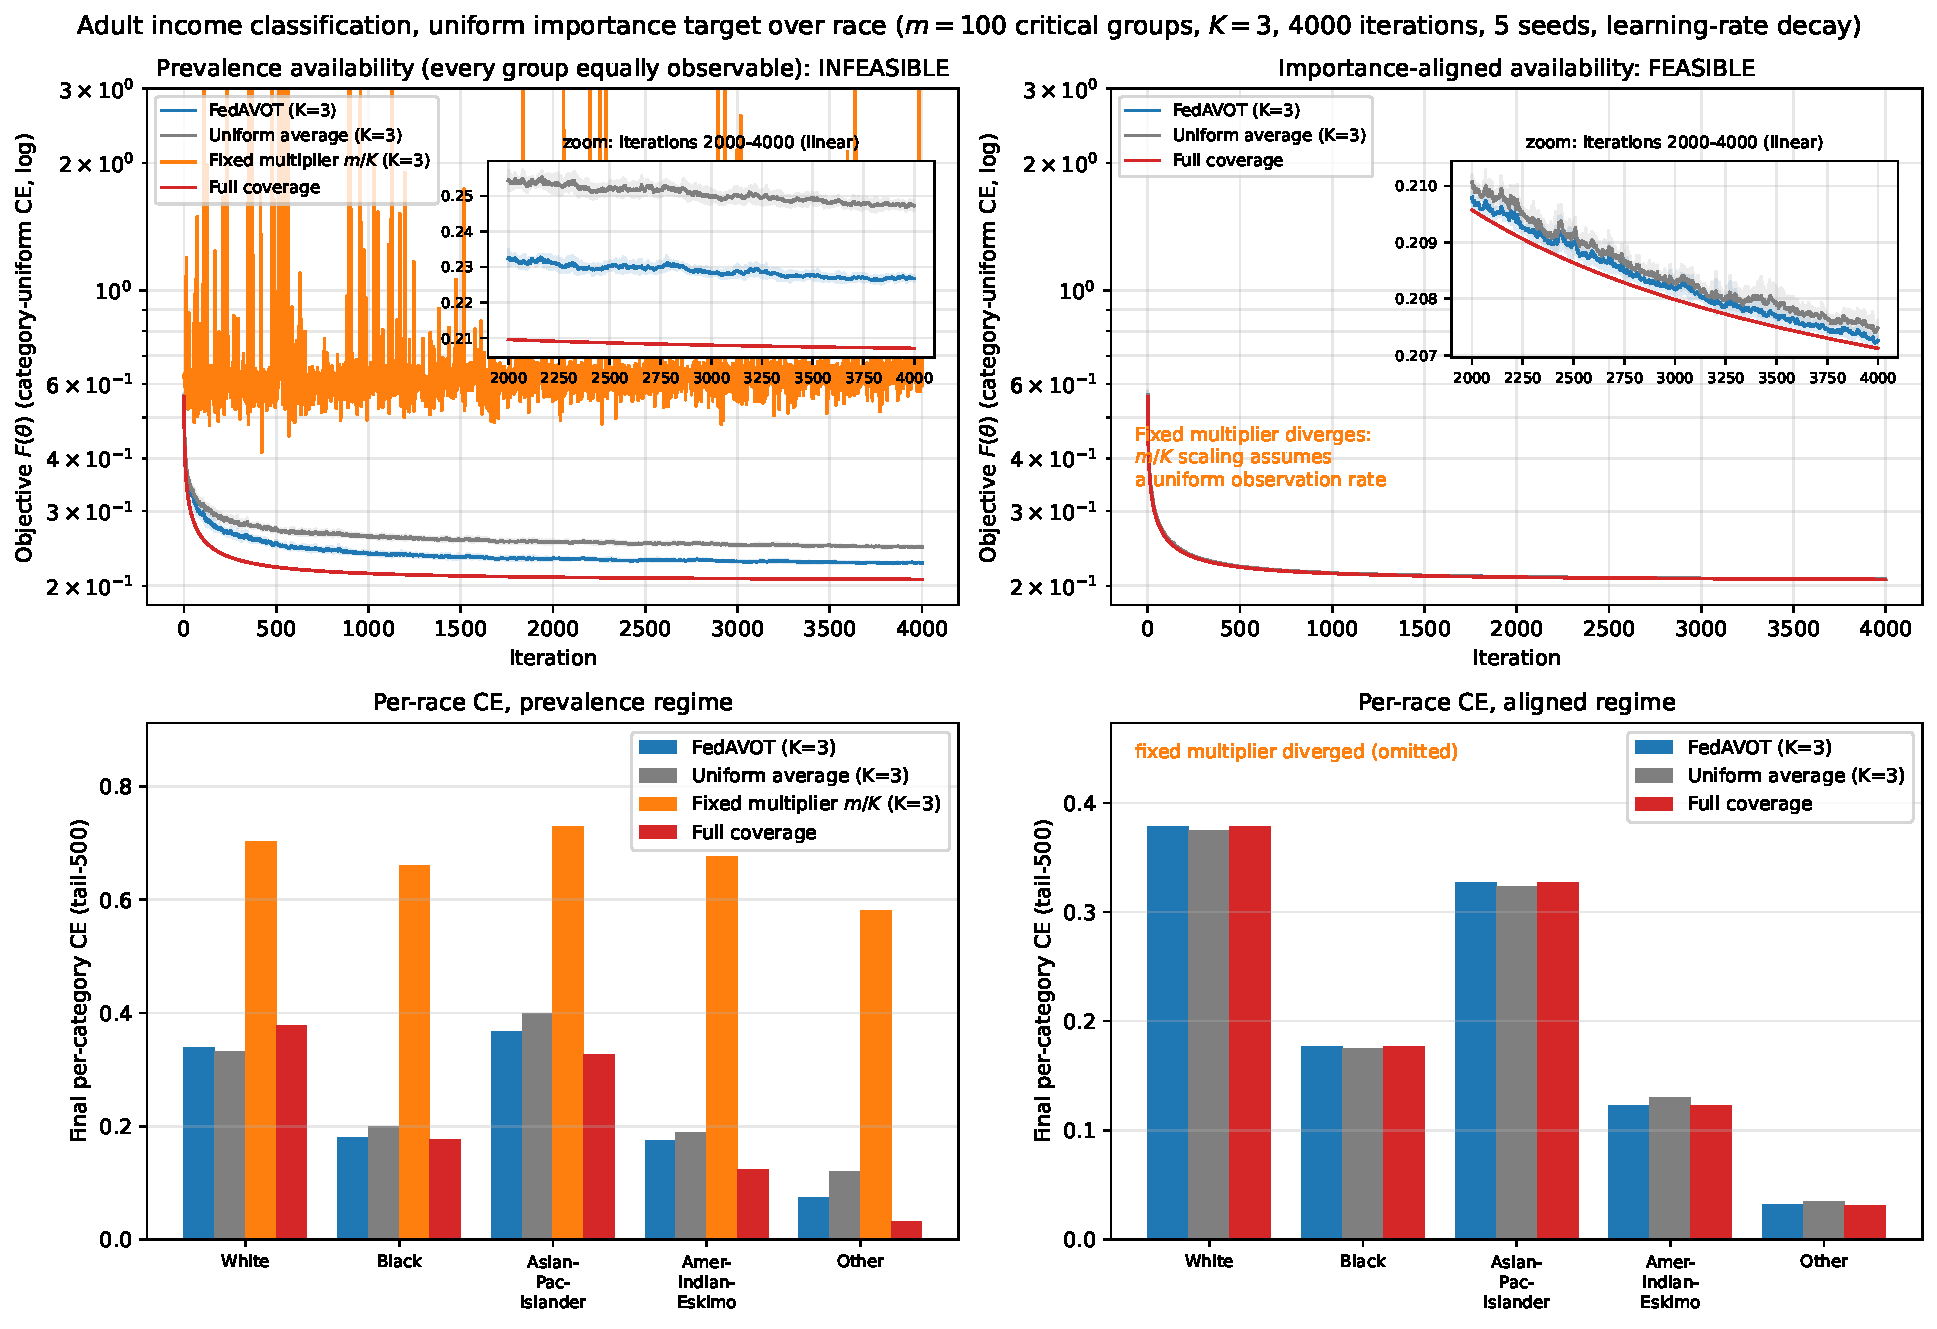
\includegraphics[width=0.8\linewidth]{adult_race_K3_4000rounds_decay.pdf}
  \caption{Adult income classification with a uniform importance target over
  race ($m=100$ groups, $K=3$, $4000$ iterations, $5$ seeds). Left column:
  prevalence availability (every group equally observable) makes the fairness
  target infeasible purely from category imbalance; FedAVOT ($0.227$) stays
  within $10\%$ of full coverage ($0.207$) and $8.5\%$ below the uniform
  average ($0.248$), while the fixed-multiplier correction is unstable, and
  the residual loss concentrates on the smallest race categories (bottom
  row). Right column: importance-aligned availability is feasible; FedAVOT
  and the uniform average both sit on top of full coverage and the
  fixed-multiplier correction diverges.}
  \label{fig:adult}
\end{figure}
% ---------------------------------------------------------------- results prose
The uniform and aligned regimes bracket the feasibility condition
(Fig.~\ref{fig:imdb-infeasible}). Under
uniform availability the transport problem is infeasible for $9$ of $100$
groups holding $31\%$ of the importance mass, and Sinkhorn scaling stalls
(row-marginal error ${\approx}9\times10^{-3}$ at termination). FedAVOT
nevertheless attains a final importance-weighted MSE of $86.06 \pm 0.21$
against $91.63 \pm 0.56$ for the uniform average and $82.95$ for full
coverage: it closes two thirds of the uniform average's excess over full
coverage, and the margin is ten seed standard deviations. In the aligned regime the same
importance distribution becomes fully feasible, Sinkhorn converges
(row-marginal error ${\approx}5\times10^{-9}$), and FedAVOT attains
$84.28 \pm 0.15$ versus $86.37 \pm 0.34$ for the uniform average, within
$1.3$ of the full-coverage value. The fixed-multiplier correction
\emph{diverges} in this regime: under availability-aligned sampling the
realized aggregation weights exceed unity in expectation, exponentially
amplifying the iterates. FedAVOT is immune by construction, since each
column of $Y$ is a convex combination.
\paragraph{Real-Data Feasibility Sweep: the Floor Gap Predicts the Sign}
Table~\ref{tab:sweep} sweeps the availability skew $\beta$ on IMDb-Wiki.
Because the task is linear regression, the minimizer of the objective each
rule actually optimizes in expectation is available in closed form (the
\emph{floor}; see the bias validation below): FedAVOT minimizes
$F_{\hat{p}}$ with the stalled surrogate $\hat{p}$, while the uniform
average minimizes $F_{\tilde{p}}$ with $\tilde{p}_i = \pi_i/K$. The gap
between the two floors is $7.0$ at $\beta=0$ and shrinks monotonically to
$0.02$ at $\beta=3$, where both surrogates starve the same groups. The
measured margin of FedAVOT over the uniform average tracks this floor gap
at every $\beta$, and its sign flips exactly where the floors cross: FedAVOT
wins by $5.6$, $3.5$, $2.1$ and $0.6$ at $\beta \le 1.5$, ties at
$\beta=2$, and trails by $2.3$ in the mirrored regime. The floor gap is a
function of $(p,q,\mathcal{E})$ alone, so it can be computed before training
to decide whether transport reweighting will help. The step-size schedule is
what makes the bias visible: at a constant step size FedAVOT trails the
uniform average at every $\beta$ (e.g.\ $95.6$ versus $94.8$ at $\beta=0$
and $116.4$ versus $108.5$ at $\beta=3$), because its per-batch weights
concentrate mass on the few important groups present, which lowers the
effective batch size and raises the variance of the iterate; the decaying
schedule removes this variance term and exposes the bias that the transport
corrects.
\begin{table}[t]
  \centering\footnotesize\setlength{\tabcolsep}{3.5pt}
  \caption{IMDb-Wiki availability sweep, $r_i \propto i^{\beta}$, $5$ seeds,
  final importance-weighted MSE (full coverage: $82.9$). $F^{\dagger}$ are the
  closed-form floors, i.e.\ the minimizers of the objective each rule
  optimizes in expectation; $\Delta$ is the measured margin of FedAVOT over
  the uniform average, which follows the floor gap and changes sign where
  the floors meet.}
  \label{tab:sweep}
  \begin{tabular}{crrrrrr}
    \hline
    $\beta$ & inf.\ mass & $F^{\dagger}_{\mathrm{FedAVOT}}$ & $F^{\dagger}_{\mathrm{unif}}$ & FedAVOT & uniform & $\Delta$ \\
    \hline
    $0$   & $31\%$ & $83.4$  & $90.4$  & $86.1$  & $91.6$  & $+5.6$ \\
    $0.5$ & $59\%$ & $90.1$  & $95.8$  & $93.2$  & $96.7$  & $+3.5$ \\
    $1$   & $70\%$ & $95.3$  & $99.0$  & $97.9$  & $99.9$  & $+2.1$ \\
    $1.5$ & $77\%$ & $98.7$  & $101.2$ & $101.2$ & $101.8$ & $+0.6$ \\
    $2$   & $82\%$ & $101.4$ & $103.0$ & $103.8$ & $103.7$ & $0.0$ \\
    $3$   & $88\%$ & $105.9$ & $105.9$ & $108.4$ & $106.1$ & $-2.3$ \\
    \hline
  \end{tabular}
\end{table}
\paragraph{Adult Results: Equal Availability Does Not Make a Fair Target Reachable}
The Adult experiment (Fig.~\ref{fig:adult}) transfers the same dichotomy
to a fairness setting. In the prevalence regime the transport is
infeasible for the five groups belonging to the three smallest race
categories ($60\%$ of the importance mass; Sinkhorn row-marginal error
stalls at ${\approx}1.7\times10^{-1}$): FedAVOT attains a category-uniform
cross-entropy of $0.2269 \pm 0.0005$ versus $0.2479 \pm 0.0009$ for the
uniform average, $0.670 \pm 0.031$ for the fixed-multiplier correction, and
$0.2073$ for full coverage, i.e., within $10\%$ of the full-coverage
objective and $8.5\%$ below the uniform average; but the unrecoverable loss
concentrates precisely on the categories the uniform target was meant to
protect (final per-category cross-entropy $0.175$ versus full coverage's
$0.123$ for Amer-Indian-Eskimo, $0.073$ versus $0.031$ for Other). In the aligned regime
($\beta=1$, row error ${\approx}3\times10^{-8}$) FedAVOT reaches
$0.2075 \pm 0.0001$, on top of the full-coverage value, and the
fixed-multiplier correction again diverges.
\bibliographystyle{plain}
\bibliography{refrences}
\end{document}